\documentclass[11pt,a4paper]{article}

\usepackage[utf8]{inputenc}
\usepackage[T1]{fontenc}
\usepackage[spanish,es-nodecimaldot]{babel}
\usepackage{lmodern}

\usepackage{graphicx}
\usepackage{geometry}
\usepackage{array}
\usepackage{amsmath}
\usepackage{titlesec}
\usepackage{hyperref}
\usepackage{fancyhdr}

\usepackage{booktabs}
\usepackage{float}

\fancyhf{}

\fancyhead[L]{\small\textit{Universidad Nacional de Ingeniería}}
\fancyhead[R]{\small\textit{2026--II}}
\renewcommand{\headrulewidth}{0.4pt}
\fancyfoot[C]{\thepage}

\geometry{
    top=2.2cm,
    bottom=1.5cm,
    left=2.5cm,
    right=2.5cm,
    headheight=14pt,
    headsep=0.5cm
}

\setlength{\parindent}{0pt}
\setlength{\parskip}{0.5em}
\pagestyle{plain}
\setcounter{secnumdepth}{2}
\setcounter{tocdepth}{2}
\addto\captionsspanish{%
    \renewcommand{\contentsname}{Contenido}%
}
\hypersetup{
    colorlinks=true,
    linkcolor=black,
    citecolor=black,
    urlcolor=blue
}

\titlespacing*{\subsection}
    {0.6cm}
    {1.5em}
    {0.8em} 

\newenvironment{subsectionbody}
{%
    \begin{list}{}{%
        \setlength{\leftmargin}{0.6cm}%
        \setlength{\rightmargin}{0cm}%
        \setlength{\topsep}{0pt}%
        \setlength{\partopsep}{0pt}%
        \setlength{\parsep}{0pt}%
        \setlength{\itemsep}{0pt}%
    }%
    \item\relax
}
{%
    \end{list}
}

\begin{document}

\begin{titlepage}

\thispagestyle{empty}

\begin{center}
{\normalsize\itshape
``Año de la Recuperación y Consolidación de la Economía Peruana''}

\vspace{0.35cm}
\resizebox{0.68\textwidth}{!}{%
    \textbf{Universidad Nacional de Ingeniería}%
}

\vspace{0.30cm}
{\Large\bfseries
Facultad de Ciencias}

\vspace{0.35cm}
{\Large\bfseries
Física II}

\vspace{0.30cm}

\includegraphics[width=4.5cm]{../figuras/imagen_uni_escudo.png}

\vspace{0.25cm}
{\Large\bfseries
Laboratorio 2}

\vspace{0.35cm}
{\Large\bfseries\itshape
Péndulo físico y teorema de Steiner}
\end{center}

\vspace{1.15cm}
\noindent
\begin{tabular*}{\textwidth}
{@{\extracolsep{\fill}}ll}
{\large\textbf{Sección:} B}
&
{\large\textbf{Día y hora:} 15/09/2026 -- 1:00 p.\,m.}
\end{tabular*}

\vspace{0.90cm}
\renewcommand{\arraystretch}{1.45}
\begin{center}
{\large
\begin{tabular}{|p{9.7cm}|p{3.4cm}|}
\hline
\textbf{Apellidos y nombres}
&
\textbf{Código}
\\
\hline
Moreno Cabanillas, Alexandra Romina
&
20251764F
\\
\hline
Mauricio Andre Polak Mory
&
20250575E
\\
\hline
Pablo Mauro Cárdenas Loyola
&
20262378E
\\
\hline
\end{tabular}
}
\end{center}

\vspace{0.85cm}
{\large\textbf{Docentes:}}
\vspace{0.35cm}
{\large
\hspace{0.6cm}

-- Cortez Reyes, Gregorio Custodio
\vspace{0.20cm}
\hspace{0.6cm}

-- Silva Vásquez, Humberto Martín
}

\vspace{0.95cm}
{\large
\textbf{Fecha de entrega del informe:}
\hspace{0.40cm}
29/09/2026
}

\vspace{1.15cm}
\begin{center}
{\huge\bfseries
2026--II}

\end{center}

\end{titlepage}

\tableofcontents

\newpage
\pagestyle{fancy}

\section{Introducción}

La participación y las contribuciones individuales de cada integrante en el desarrollo de la
experiencia y la elaboración del presente informe se detallan en la sección de anexos.

El estudio del movimiento oscilatorio ha desempeñado un papel fundamental
en el desarrollo de la mecánica clásica y en la comprensión del movimiento
de los cuerpos bajo la acción de la gravedad. Durante el siglo XVII, el
análisis del péndulo adquirió especial importancia debido a su aplicación
en la medición precisa del tiempo. Christiaan Huygens desarrolló en 1656
uno de los primeros relojes de péndulo funcionales y, posteriormente,
publicó en 1673 su obra \textit{Horologium Oscillatorium}, en la que
presentó un estudio matemático del movimiento pendular y abordó el problema
del centro de oscilación de cuerpos rígidos.

Estos estudios permitieron extender el análisis desde el péndulo simple
idealizado hacia sistemas en los que la masa se encuentra distribuida en
todo el cuerpo. Surge así el estudio del péndulo físico o compuesto, cuyo
período de oscilación depende no solamente de la posición de su eje de
suspensión, sino también de la distribución de su masa. Esta propiedad se
caracteriza mediante el momento de inercia, magnitud que desempeña en la
dinámica rotacional un papel análogo al de la masa en el movimiento
traslacional. El trabajo de Huygens sobre los centros de oscilación ya
contenía resultados relacionados con lo que actualmente se expresa
mediante momentos de inercia respecto de ejes paralelos.

En la formulación moderna, la relación entre el momento de inercia respecto
a un eje que pasa por el centro de masa y otro eje paralelo separado de
este una determinada distancia se conoce como teorema de los ejes paralelos
o teorema de Steiner. Su aplicación al péndulo físico permite relacionar
el período de oscilación con la masa del cuerpo, la posición de su centro
de gravedad y su momento de inercia, proporcionando así un procedimiento
experimental para estudiar la distribución de masa de un cuerpo rígido.

En la presente experiencia se estudia el movimiento oscilatorio de una
barra metálica homogénea provista de varios agujeros, los cuales permiten
modificar la posición del eje de suspensión. Para cada posición se mide
el tiempo correspondiente a un determinado número de oscilaciones y la
distancia entre el eje de suspensión y el centro de gravedad de la barra.
A partir de estas mediciones se determinarán los períodos y los
correspondientes momentos de inercia, analizando su dependencia con la
posición del eje de oscilación y contrastando los resultados experimentales
con las relaciones teóricas del péndulo físico y del teorema de Steiner.

\newpage

\section{Objetivos}

\subsection{Objetivo general}

Determinar experimentalmente los períodos de oscilación de un péndulo
físico y, a partir de ellos, calcular los momentos de inercia asociados
a diferentes ejes de suspensión, analizando su relación con la posición
del eje de oscilación mediante el teorema de Steiner.

\subsection{Objetivos específicos}

\begin{itemize}

    \item Medir el tiempo empleado por una barra metálica para realizar
    un determinado número de oscilaciones respecto a diferentes ejes de
    suspensión.

    \item Determinar el período de oscilación correspondiente a cada
    posición del eje de suspensión.

    \item Determinar experimentalmente los momentos de inercia de la barra
    respecto a los diferentes ejes de oscilación.

    \item Analizar la variación del período de oscilación en función de la
    distancia entre el eje de suspensión y el centro de gravedad de la
    barra.

    \item Verificar experimentalmente el teorema de Steiner mediante el
    análisis de la relación entre el momento de inercia y el cuadrado de
    la distancia entre el eje de oscilación y el centro de gravedad.

    \item Determinar experimentalmente el momento de inercia de la barra
    respecto a un eje que pasa por su centro de masa.

    \item Comparar el momento de inercia obtenido experimentalmente con
    el calculado mediante la expresión analítica correspondiente a una
    barra homogénea.

\end{itemize}

\newpage
\section{Fundamentos teóricos}

\subsection{Péndulo físico}
\begin{subsectionbody}

A diferencia del péndulo simple, su masa se encuentra distribuida en un volumen finito,
por lo que su dinámica depende del momento de inercia respecto al eje
de suspensión.

Según Alonso y Finn (1995, p.~278), \textit{``Un péndulo físico (o
compuesto) es un sólido rígido que puede oscilar libremente alrededor
de un eje horizontal bajo la acción de la gravedad''}.

Sea $O$ el eje de suspensión y $\ell$ la distancia desde dicho eje
hasta el centro de masa. Cuando el cuerpo se separa un ángulo $\theta$
de la posición de equilibrio, el peso $Mg$ genera un torque restaurador:

\[
\tau=-Mg\ell\sin\theta
\]

El signo negativo indica que el torque se opone al desplazamiento
angular. Para oscilaciones pequeñas,

\[
\sin\theta\simeq\theta,
\]

por lo que

\[
\tau\simeq-Mg\ell\theta.
\]

donde:

\hspace*{0.5cm}$\tau$: torque respecto al eje de suspensión
($\mathrm{N\,m}$).\\
\hspace*{0.5cm}$M$: masa del cuerpo ($\mathrm{kg}$).\\
\hspace*{0.5cm}$g$: aceleración de la gravedad ($\mathrm{m/s^2}$).\\
\hspace*{0.5cm}$\ell$: distancia del eje de suspensión al centro de masa
($\mathrm{m}$).\\
\hspace*{0.5cm}$\theta$: desplazamiento angular ($\mathrm{rad}$).

\end{subsectionbody}


\subsection{Ecuación de movimiento y período del péndulo físico}
\begin{subsectionbody}

El movimiento del péndulo físico se obtiene aplicando la segunda ley
de Newton para la rotación. Para pequeñas amplitudes, el torque
restaurador es aproximadamente proporcional al desplazamiento angular,
por lo que el sistema puede describirse como un M.A.S.

Según Sears, Zemansky, Young y Freedman (2009, p.~438),
\textit{``si $\theta$ es pequeño, podemos aproximar $\sin\theta$ con
$\theta$ en radianes''}.

La ecuación fundamental de la dinámica rotacional es

\[
\sum\tau=I_1\alpha,
\]

donde la aceleración angular está definida por

\[
\alpha=\frac{d^2\theta}{dt^2}.
\]

Sustituyendo el torque restaurador,

\[
-Mg\ell\sin\theta
=
I_1\frac{d^2\theta}{dt^2}.
\]

Para pequeñas oscilaciones,

\[
-Mg\ell\theta
=
I_1\frac{d^2\theta}{dt^2}.
\]

Reordenando,

\[
\frac{d^2\theta}{dt^2}
+
\frac{Mg\ell}{I_1}\theta
=0.
\]

La ecuación característica del movimiento armónico simple es

\[
\frac{d^2\theta}{dt^2}
+
\omega^2\theta
=0.
\]

Por comparación,

\[
\omega^2=\frac{Mg\ell}{I_1}.
\]

Como

\[
\omega=\frac{2\pi}{T},
\]

se obtiene el período del péndulo físico:

\begin{equation}
\boxed{
T=2\pi\sqrt{\frac{I_1}{Mg\ell}}
}
\label{eq:periodo_pendulo_fisico}
\end{equation}

donde:

\hspace*{0.5cm}$I_1$: momento de inercia respecto al eje de suspensión
($\mathrm{kg\,m^2}$).\\
\hspace*{0.5cm}$\alpha$: aceleración angular ($\mathrm{rad/s^2}$).\\
\hspace*{0.5cm}$\omega$: frecuencia angular ($\mathrm{rad/s}$).\\
\hspace*{0.5cm}$T$: período de oscilación ($\mathrm{s}$).\\
\hspace*{0.5cm}$t$: tiempo ($\mathrm{s}$).

\end{subsectionbody}

\subsection{Momento de inercia}
\begin{subsectionbody}

El momento de inercia cuantifica la resistencia de un cuerpo a
modificar su estado de rotación respecto de un eje determinado.

Según Giancoli (2006, p.~207), el momento de inercia
\textit{``juega el mismo papel para el movimiento de rotación que
desempeña la masa para el movimiento de traslación''}.

Para un sistema continua,

\[
I=\int r^2\,dm.
\]

En el presente experimento, el momento de inercia respecto al eje de
suspensión puede determinarse a partir del período, elevando al cuadrado
la ecuación \eqref{eq:periodo_pendulo_fisico} y despejando,

\begin{equation}
\boxed{
I_1=\frac{Mg\ell T^2}{4\pi^2}
}
\label{eq:momento_experimental}
\end{equation}

Esta expresión permite determinar experimentalmente el momento de
inercia para cada posición del eje de suspensión.
\end{subsectionbody}


\subsection{Teorema de Steiner o de los ejes paralelos}
\begin{subsectionbody}

El teorema de Steiner relaciona el momento de inercia respecto a un
eje que atraviesa el centro de masa con el correspondiente a cualquier
eje paralelo.

Según Tipler y Mosca (2008, p.~297), este teorema
\textit{``relaciona el momento de inercia respecto a un eje que pasa
por el centro de masas de un objeto, con el momento de inercia respecto
a otro eje paralelo al primero''}.

Para demostrarlo, considérese un cuerpo cuyo centro de masa constituye
el origen del sistema de coordenadas $(x,y)$. Sea un segundo eje
paralelo desplazado respecto al primero, con componentes $a$ y $b$.
El momento de inercia respecto al eje desplazado es

\[
I_1=
\int
\left[
(x-a)^2+(y-b)^2
\right]dm.
\]

Desarrollando,

\[
\begin{aligned}
I_1={}&
\int(x^2+y^2)\,dm
-2a\int x\,dm
-2b\int y\,dm \\
&+(a^2+b^2)\int dm.
\end{aligned}
\]

Por definición del centro de masa,

\[
\int x\,dm=0,
\qquad
\int y\,dm=0.
\]

Además,

\[
I_G=\int(x^2+y^2)\,dm,
\]

\[
\int dm=M,
\]

y, si la distancia entre los dos ejes es $\ell$,

\[
\ell^2=a^2+b^2.
\]

Por tanto,

\begin{equation}
\boxed{
I_1=I_G+M\ell^2
}
\label{eq:steiner}
\end{equation}

donde:

\hspace*{0.5cm}$I_G$: momento de inercia respecto al eje que pasa por
el centro de masa ($\mathrm{kg\,m^2}$).\\
\hspace*{0.5cm}$a,b$: componentes del desplazamiento entre los ejes
($\mathrm{m}$).

\end{subsectionbody}

\subsection{Relación entre \texorpdfstring{$I_1$}{I1} y
\texorpdfstring{$\ell^2$}{l2}}

\begin{subsectionbody}

El teorema de Steiner permite determinar experimentalmente tanto el
momento de inercia respecto al centro de masa como la masa de la barra
mediante una relación lineal.

Medina Guzmán (2007, cap.~7, p.~2) presenta el teorema de Steiner
mediante la relación

\[
I_0=I_{CM}+Md^2.
\]

Para la notación empleada en este experimento,

\[
I_1=M\ell^2+I_G.
\]

Comparando con la ecuación de una recta,

\[
y=mx+c,
\]

se establecen las correspondencias

\[
y=I_1,
\qquad
x=\ell^2,
\]

de donde

\[
\text{pendiente}=M,
\qquad
\text{intercepto}=I_G.
\]

En consecuencia, el ajuste lineal de los valores experimentales de
$I_1$ en función de $\ell^2$ permite obtener experimentalmente $M$ e
$I_G$.

\end{subsectionbody}

\subsection{Momento de inercia teórico de la barra}
\begin{subsectionbody}

Para contrastar el resultado experimental es necesario calcular el
momento de inercia geométrico de la barra respecto a un eje
perpendicular a su superficie que atraviesa su centro de masa.

Halliday, Resnick y Walker desarrollan el caso de una placa rectangular
uniforme, cuyo momento de inercia respecto a un eje perpendicular a la
placa y que pasa por su centro depende de sus dimensiones geométricas.

Para una barra rectangular de longitud $L$ y ancho $b$,

\begin{equation}
\boxed{
I_{G,\mathrm{teo}}
=
\frac{1}{12}M\left(L^2+b^2\right)
}
\label{eq:momento_teorico}
\end{equation}

donde:

\hspace*{0.5cm}$I_{G,\mathrm{teo}}$: momento de inercia teórico respecto
al centro de masa ($\mathrm{kg\,m^2}$).\\
\hspace*{0.5cm}$L$: longitud de la barra ($\mathrm{m}$).\\
\hspace*{0.5cm}$b$: ancho de la barra ($\mathrm{m}$).

\end{subsectionbody}

\subsection{Período mínimo del péndulo físico}

\begin{subsectionbody}

La posición del eje de suspensión modifica simultáneamente el torque
gravitacional y el momento de inercia del sistema. En consecuencia,
existe una distancia determinada entre el eje y el centro de masa para
la cual el período alcanza un mínimo.

Sustituyendo el teorema de Steiner en la expresión del período,

\[
T=
2\pi
\sqrt{
\frac{I_G+M\ell^2}{Mg\ell}
}.
\]

Elevando al cuadrado,

\[
T^2=
\frac{4\pi^2}{g}
\left(
\ell+\frac{I_G}{M\ell}
\right).
\]

El mínimo de $T$ coincide con el mínimo de $T^2$, por lo que

\[
\frac{d(T^2)}{d\ell}=0.
\]

Derivando,

\[
\frac{4\pi^2}{g}
\left(
1-\frac{I_G}{M\ell^2}
\right)=0.
\]

Entonces,

\[
\ell^2=\frac{I_G}{M}.
\]

Por tanto,

\begin{equation}
\boxed{
\ell_{\min}=
\sqrt{\frac{I_G}{M}}
}
\label{eq:distancia_periodo_minimo}
\end{equation}

donde:

\hspace*{0.5cm}$\ell_{\min}$: distancia al centro de masa correspondiente
al período mínimo ($\mathrm{m}$).

\end{subsectionbody}

\subsection{Propagación de incertidumbres}

\begin{subsectionbody}

Las magnitudes principales del experimento, como $T$, $I_1$,
$\ell^2$ e $I_{G,\mathrm{teo}}$, son obtenidas indirectamente a partir
de cantidades medidas. Por ello, sus incertidumbres deben determinarse
mediante propagación.

Para una magnitud

\[
Q=f(x_1,x_2,\ldots,x_n),
\]

si las variables son independientes, la incertidumbre combinada está
dada por

\[
u_Q=
\sqrt{
\sum_{i=1}^{n}
\left(
\frac{\partial Q}{\partial x_i}u_{x_i}
\right)^2
}.
\]

Para el momento de inercia experimental,

\[
I_1=\frac{Mg\ell T^2}{4\pi^2},
\]

considerando $g$ constante,

\[
u_{I_1}
=
\sqrt{
\left(
\frac{\partial I_1}{\partial M}u_M
\right)^2
+
\left(
\frac{\partial I_1}{\partial\ell}u_\ell
\right)^2
+
\left(
\frac{\partial I_1}{\partial T}u_T
\right)^2
}.
\]

Las derivadas parciales son

\[
\frac{\partial I_1}{\partial M}
=
\frac{g\ell T^2}{4\pi^2},
\]

\[
\frac{\partial I_1}{\partial\ell}
=
\frac{MgT^2}{4\pi^2},
\]

\[
\frac{\partial I_1}{\partial T}
=
\frac{Mg\ell T}{2\pi^2}.
\]

Por tanto,

\begin{equation}
\boxed{
\frac{u_{I_1}}{I_1}
=
\sqrt{
\left(\frac{u_M}{M}\right)^2
+
\left(\frac{u_\ell}{\ell}\right)^2
+
\left(2\frac{u_T}{T}\right)^2
}
}
\label{eq:incertidumbre_momento}
\end{equation}

Para la variable $\ell^2$ utilizada en la gráfica del teorema de
Steiner,

\begin{equation}
\boxed{
u_{\ell^2}=2\ell u_\ell
}
\label{eq:incertidumbre_l2}
\end{equation}

Asimismo, para $T^2$,

\begin{equation}
\boxed{
u_{T^2}=2T u_T
}
\label{eq:incertidumbre_T2}
\end{equation}

donde:

\hspace*{0.5cm}$u_Q$: incertidumbre de la magnitud indirecta $Q$.\\
\hspace*{0.5cm}$u_M$: incertidumbre de la masa ($\mathrm{kg}$).\\
\hspace*{0.5cm}$u_\ell$: incertidumbre de la distancia ($\mathrm{m}$).\\
\hspace*{0.5cm}$u_T$: incertidumbre del período ($\mathrm{s}$).\\
\hspace*{0.5cm}$u_{I_1}$: incertidumbre del momento de inercia
($\mathrm{kg\,m^2}$).

\end{subsectionbody}

\newpage
\section{Materiales y equipos}

\subsection{Elementos de montaje y soporte}

Elementos empleados para sostener y fijar el sistema durante la experiencia.

\begin{itemize}
    \item \textbf{Mordaza:} utilizada para fijar el montaje.
    \item \textbf{Bastidor en forma de A:} estructura empleada como soporte del sistema oscilante.
\end{itemize}

\subsection{Instrumentos de medición y adquisición de datos}

Instrumentos utilizados para medir las magnitudes experimentales.

\begin{itemize}
    \item \textbf{Cronómetro digital:} resolución de $0.01\,\mathrm{s}$.
    \item \textbf{Regla milimétrica:} resolución de $0.05\,\mathrm{cm}$.
\end{itemize}

\subsection{Componentes del sistema}

Elementos que constituyen el sistema físico sometido a estudio.

\begin{itemize}
    \item \textbf{Barra de hierro con agujeros:} posee 19 agujeros circulares, masa de $1.8402\,\mathrm{kg}$, longitud de $1.001\,\mathrm{m}$ y ancho de $0.037\,\mathrm{m}$.
\end{itemize}

\begin{figure}[ht]
    \centering
    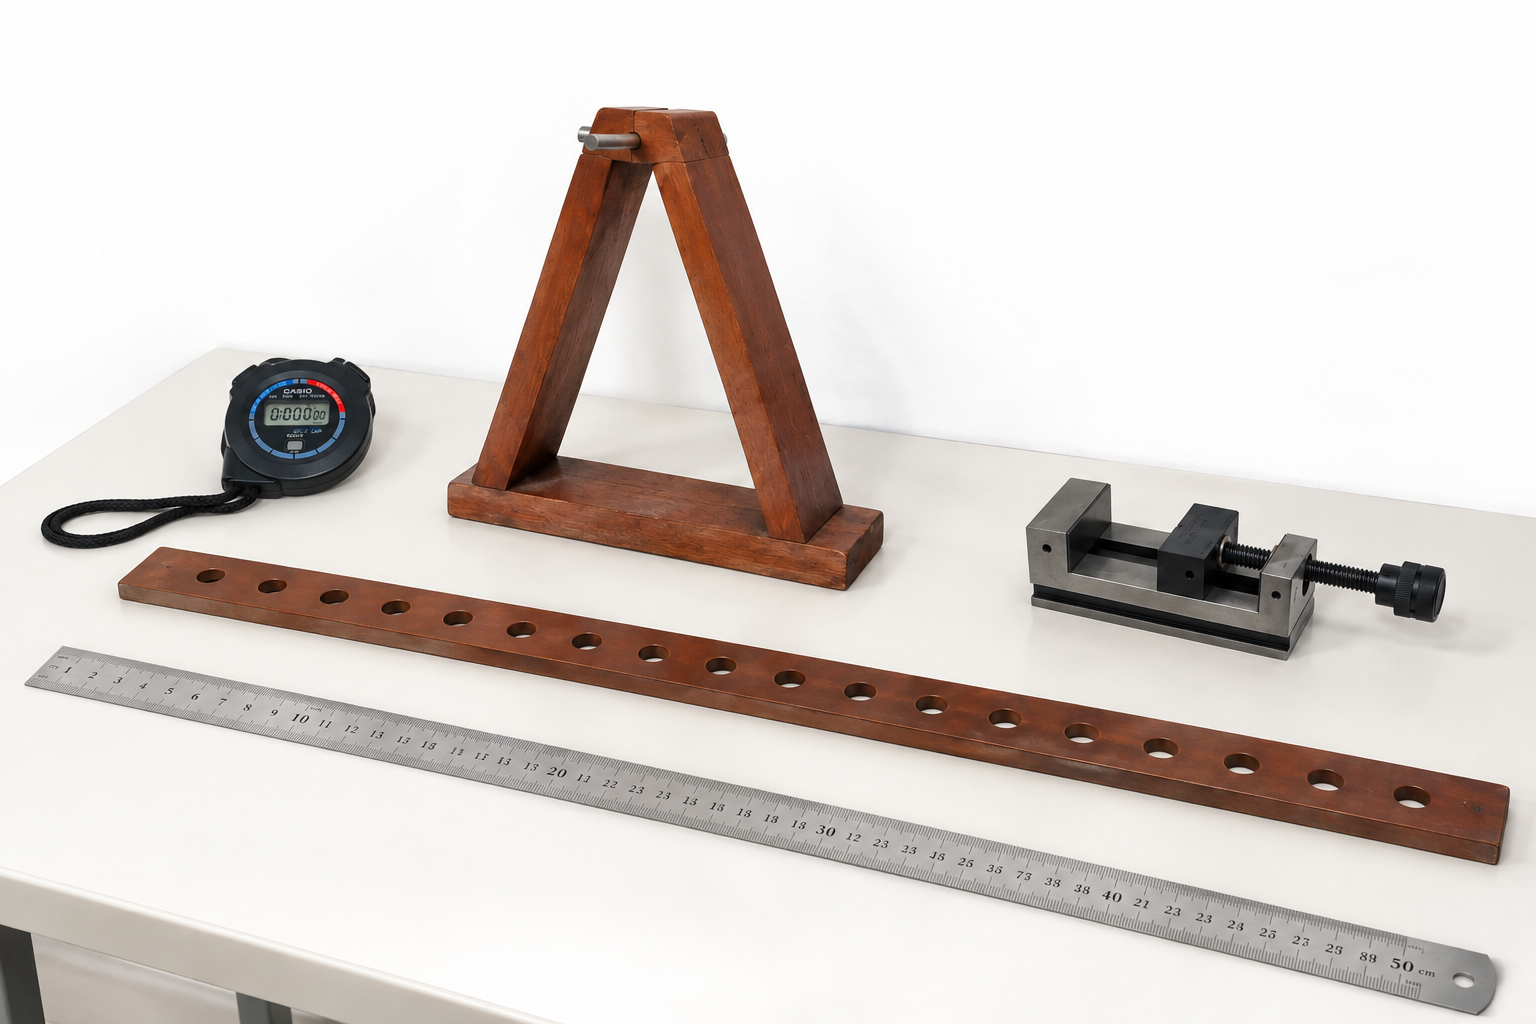
\includegraphics[width=0.90\textwidth]{../figuras/Materiales.png}
    \caption{Materiales y equipos empleados en el estudio experimental del péndulo físico.}
    \label{fig:materiales_equipos}
\end{figure}

\newpage
\section{Procedimiento experimental}

\begin{enumerate}

    \item Se instaló el bastidor en forma de A sobre la mesa de trabajo y se aseguró el montaje mediante la mordaza, verificando que el sistema permaneciera estable durante las oscilaciones de la barra.

    \item Se determinó experimentalmente el \textbf{centro de masa de la barra}, colocándola horizontalmente sobre el punto de apoyo y variando su posición hasta alcanzar una condición de equilibrio. Esta posición se tomó como referencia para las posteriores mediciones de distancia.

    \item La barra se suspendió verticalmente utilizando uno de sus agujeros como eje de oscilación. A continuación, se desplazó ligeramente de su posición de equilibrio, manteniendo una amplitud angular no mayor de $15^\circ$.

    \item Para cada agujero utilizado como punto de suspensión, se midió con la regla la distancia $\ell$ comprendida entre el eje de oscilación y el centro de masa previamente determinado.

    \item Se dejó oscilar libremente la barra y, mediante el cronómetro digital, se registró el tiempo correspondiente a \textbf{20 oscilaciones completas}. Para los puntos de suspensión más próximos al centro de masa se consideraron \textbf{10 oscilaciones}.

    \item La medición del tiempo se realizó \textbf{tres veces para cada posición del eje de suspensión}, manteniendo las mismas condiciones experimentales. Estos valores se utilizaron posteriormente para determinar el período promedio correspondiente a cada distancia $\ell$.

    \item Finalmente, se registraron las dimensiones y la masa de la barra. Estos datos, junto con los períodos experimentales, se emplearon para determinar los momentos de inercia y analizar su dependencia con la posición del eje de oscilación.

\end{enumerate}

\begin{figure}[ht]
    \centering
    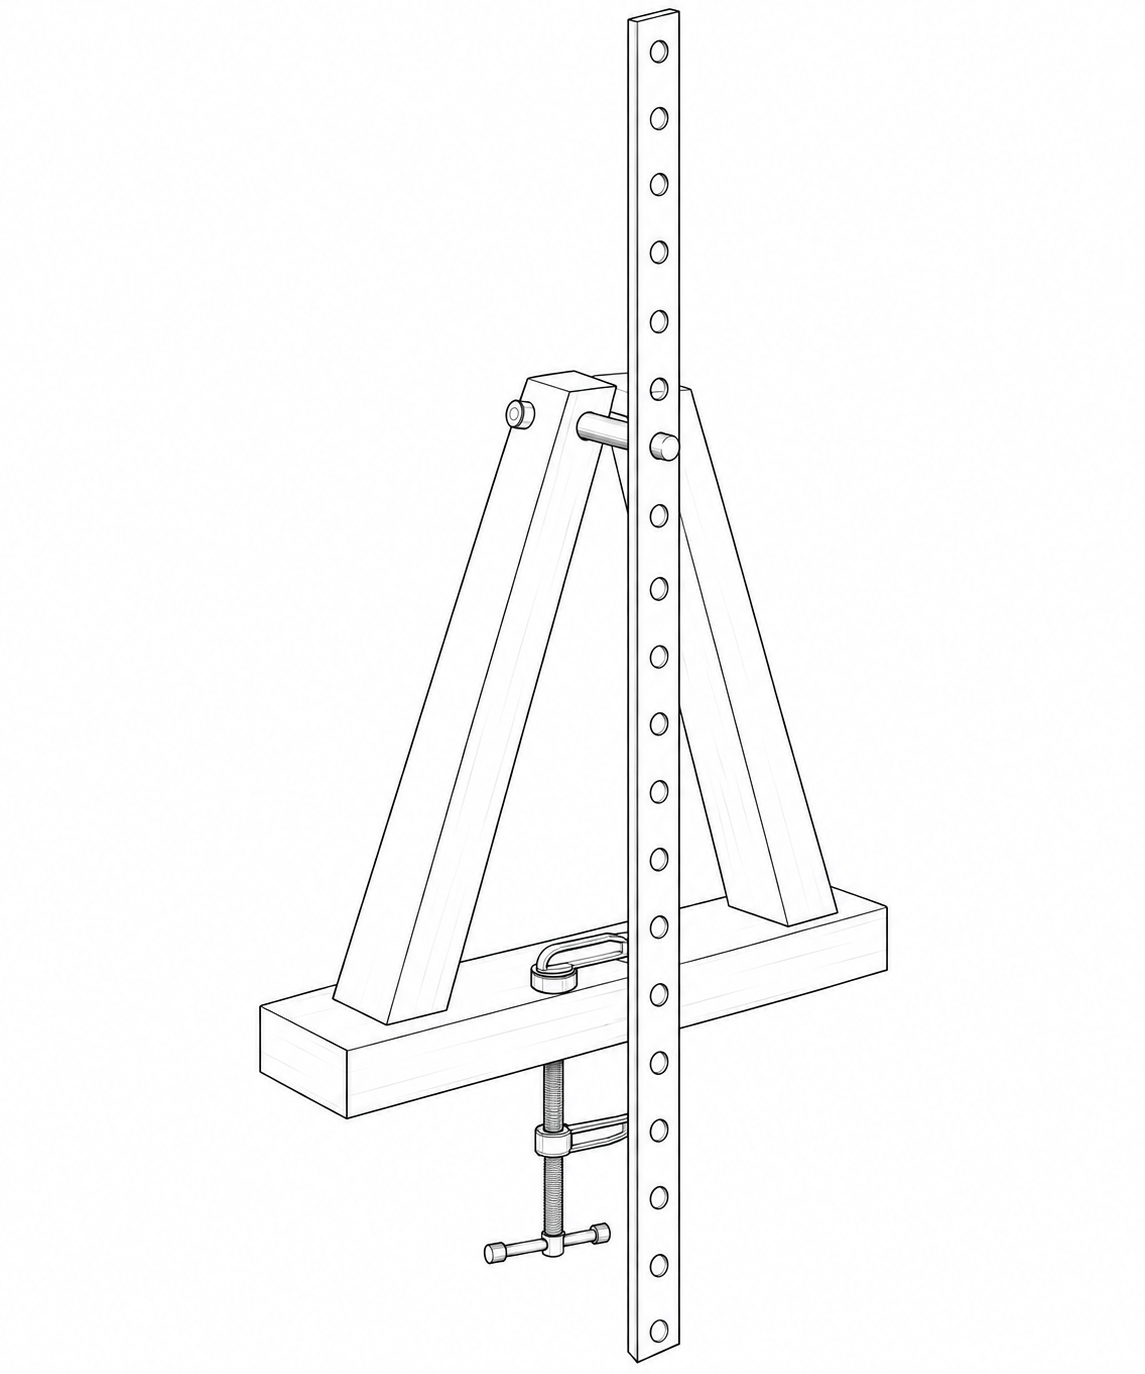
\includegraphics[width=0.55\textwidth]{../figuras/montaje.png}
    \caption{Esquema del montaje experimental empleado para el estudio del péndulo físico.}
    \label{fig:montaje_experimental}
\end{figure}

\newpage
\section{Datos experimentales}

A continuación se presentarán los datos tomados en el laboratorio.

\vspace{0.2cm}

\begin{table}[H]
    \centering
    \small
    \renewcommand{\arraystretch}{0.92}
    \setlength{\tabcolsep}{9pt}

    \begin{tabular}{cccccc}
        \toprule
        \textbf{Hueco} &
        $\boldsymbol{\ell}$ \textbf{(m)} &
        $\boldsymbol{t_1}$ \textbf{(s)} &
        $\boldsymbol{t_2}$ \textbf{(s)} &
        $\boldsymbol{t_3}$ \textbf{(s)} &
        $\boldsymbol{N}$ \\
        \midrule

        1  & 0.503 & 33.62 & 33.62 & 33.62 & 20 \\
        2  & 0.454 & 32.90 & 32.82 & 32.90 & 20 \\
        3  & 0.403 & 32.22 & 32.06 & 32.22 & 20 \\
        4  & 0.353 & 32.01 & 31.89 & 31.64 & 20 \\
        5  & 0.304 & 31.72 & 31.82 & 31.62 & 20 \\
        6  & 0.253 & 32.11 & 32.21 & 32.33 & 20 \\
        7  & 0.204 & 33.24 & 33.24 & 32.92 & 20 \\
        8  & 0.153 & 17.71 & 17.99 & 17.76 & 10 \\
        9  & 0.102 & 20.55 & 20.37 & 20.28 & 10 \\
        10 & 0.053 & 26.44 & 27.21 & 26.70 & 10 \\

        \bottomrule
    \end{tabular}

    \caption{Mediciones experimentales correspondientes al primer integrante.}
    \label{tab:datos_integrante1}
\end{table}

\vspace{-0.25cm}


\begin{table}[H]
    \centering
    \small
    \renewcommand{\arraystretch}{0.92}
    \setlength{\tabcolsep}{9pt}

    \begin{tabular}{cccccc}
        \toprule
        \textbf{Hueco} &
        $\boldsymbol{\ell}$ \textbf{(m)} &
        $\boldsymbol{t_1}$ \textbf{(s)} &
        $\boldsymbol{t_2}$ \textbf{(s)} &
        $\boldsymbol{t_3}$ \textbf{(s)} &
        $\boldsymbol{N}$ \\
        \midrule

        1  & 0.503 & 33.57 & 33.34 & 33.28 & 20 \\
        2  & 0.454 & 32.78 & 32.96 & 32.65 & 20 \\
        3  & 0.403 & 32.30 & 32.31 & 32.91 & 20 \\
        4  & 0.353 & 31.69 & 32.11 & 31.96 & 20 \\
        5  & 0.304 & 31.94 & 31.90 & 32.40 & 20 \\
        6  & 0.253 & 31.95 & 32.31 & 32.63 & 20 \\
        7  & 0.204 & 33.28 & 33.42 & 33.14 & 20 \\
        8  & 0.153 & 17.01 & 17.63 & 17.76 & 10 \\
        9  & 0.102 & 20.33 & 20.53 & 20.53 & 10 \\
        10 & 0.053 & 26.86 & 27.04 & 26.76 & 10 \\

        \bottomrule
    \end{tabular}

    \caption{Mediciones experimentales correspondientes al segundo integrante.}
    \label{tab:datos_integrante2}
\end{table}

\vspace{-0.25cm}

\begin{table}[H]
    \centering
    \small
    \renewcommand{\arraystretch}{0.92}
    \setlength{\tabcolsep}{9pt}

    \begin{tabular}{cccccc}
        \toprule
        \textbf{Hueco} &
        $\boldsymbol{\ell}$ \textbf{(m)} &
        $\boldsymbol{t_1}$ \textbf{(s)} &
        $\boldsymbol{t_2}$ \textbf{(s)} &
        $\boldsymbol{t_3}$ \textbf{(s)} &
        $\boldsymbol{N}$ \\
        \midrule

        1  & 0.503 & 33.41 & 33.17 & 31.58 & 20 \\
        2  & 0.454 & 30.74 & 30.82 & 31.62 & 20 \\
        3  & 0.403 & 32.22 & 32.33 & 32.34 & 20 \\
        4  & 0.353 & 31.63 & 31.99 & 32.01 & 20 \\
        5  & 0.304 & 31.96 & 31.90 & 31.94 & 20 \\
        6  & 0.253 & 31.95 & 32.30 & 31.60 & 20 \\
        7  & 0.204 & 33.20 & 33.52 & 33.20 & 20 \\
        8  & 0.153 & 17.00 & 16.91 & 17.56 & 10 \\
        9  & 0.102 & 20.32 & 20.43 & 20.54 & 10 \\
        10 & 0.053 & 26.70 & 27.05 & 27.30 & 10 \\

        \bottomrule
    \end{tabular}

    \caption{Mediciones experimentales correspondientes al tercer integrante.}
    \label{tab:datos_integrante3}
\end{table}

\newpage
\section{Cálculos y resultados}

A partir de los datos experimentales se calcularon los períodos de
oscilación y los momentos de inercia correspondientes a cada posición
del eje de suspensión. A continuación se desarrolla el procedimiento
para el primer conjunto de datos. Los otros dos conjuntos fueron
procesados de manera análoga mediante Python.

\subsection{Determinación del período de oscilación}

Para cada posición del eje de suspensión se realizaron tres mediciones
del tiempo. El período promedio se calculó mediante

\[
T=
\frac{t_1+t_2+t_3}{3N}.
\]


Aplicando a las demás posiciones se obtuvieron
los siguientes resultados.

\begin{table}[H]
    \centering
    \small
    \renewcommand{\arraystretch}{1.05}

    \begin{tabular}{ccc}
        \toprule
        \textbf{Hueco} &
        $\boldsymbol{\ell}$ \textbf{(m)} &
        $\boldsymbol{T}$ \textbf{(s)} \\
        \midrule
        1  & 0.503 & 1.6810 \\
        2  & 0.454 & 1.6437 \\
        3  & 0.403 & 1.6083 \\
        4  & 0.353 & 1.5923 \\
        5  & 0.304 & 1.5860 \\
        6  & 0.253 & 1.6108 \\
        7  & 0.204 & 1.6567 \\
        8  & 0.153 & 1.7820 \\
        9  & 0.102 & 2.0400 \\
        10 & 0.053 & 2.6783 \\
        \bottomrule
    \end{tabular}

    \caption{Períodos obtenidos para el primer conjunto de datos.}
    \label{tab:periodos_integrante1}
\end{table}

\subsection{Período en función de la distancia}

Los períodos calculados se representaron en función de la distancia
$\ell$ entre el eje de suspensión y el centro de masa.

\begin{figure}[!htb]
    \centering
    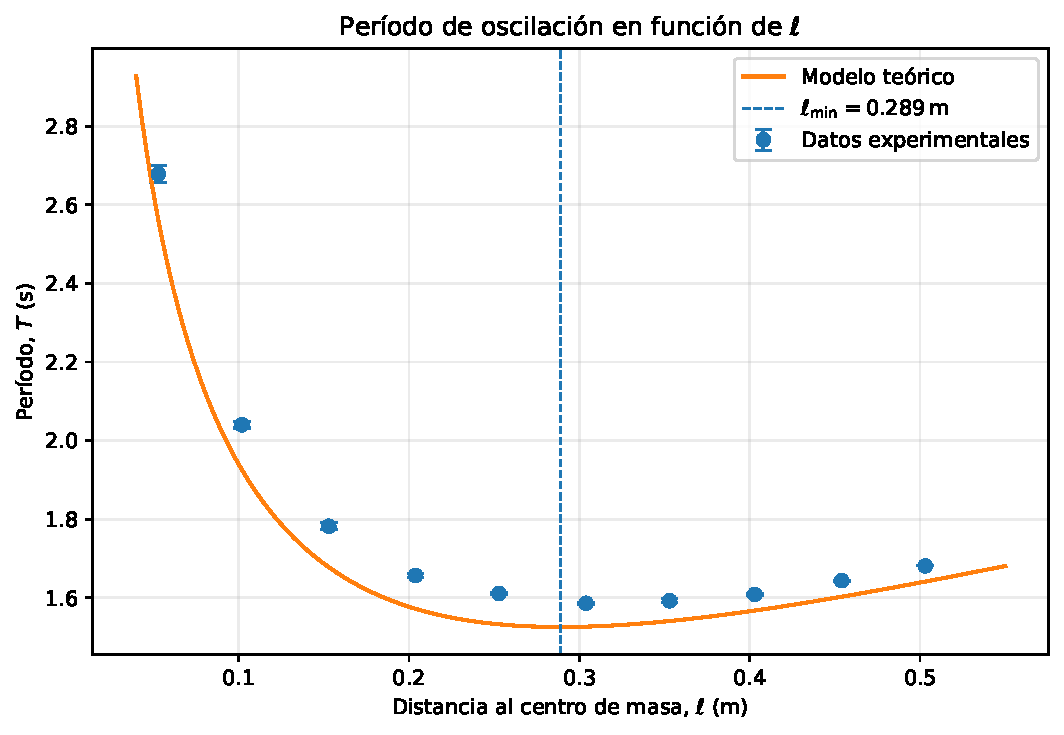
\includegraphics[width=0.58\textwidth]
    {../figuras/periodo_vs_distancia_integrante1.pdf}
    \caption{Período de oscilación en función de la distancia $\ell$ para el primer conjunto de datos.}
    \label{fig:periodo_integrante1}
\end{figure}

\newpage
El menor período entre las posiciones medidas fue

\[
\boxed{
T_{\min,\mathrm{exp}}=1.5860\,\mathrm{s}
}
\]

para

\[
\boxed{
\ell=0.304\,\mathrm{m}
}.
\]

Teóricamente, la posición correspondiente al período mínimo está dada por

\[
\ell_{\min}=\sqrt{\frac{I_G}{M}}.
\]

Para la barra empleada,

\[
I_{G,\mathrm{teo}}
=
\frac{1}{12}M(L^2+b^2)
=
0.153867\,\mathrm{kg\,m^2}.
\]

Por tanto,

\[
\boxed{
\ell_{\min,\mathrm{teo}}
=
0.289161\,\mathrm{m}
}
\]

y el período mínimo teórico correspondiente es

\[
\boxed{
T_{\min,\mathrm{teo}}
=
1.525564\,\mathrm{s}
}.
\]

El mínimo experimental se encuentra próximo al valor predicho
teóricamente.

\subsection{Determinación experimental del momento de inercia}

Para cada posición del eje de suspensión se calculó el momento de
inercia mediante

\[
I_1=
\frac{Mg\ell T^2}{4\pi^2}.
\]

Los resultados obtenidos para todas las posiciones se presentan en el
siguiente cuadro.

\begin{table}[H]
    \centering
    \small
    \renewcommand{\arraystretch}{1.05}
    \setlength{\tabcolsep}{9pt}

    \begin{tabular}{cccc}
        \toprule
        $\boldsymbol{\ell}$ \textbf{(m)} &
        $\boldsymbol{T^2}$ \textbf{(s$^2$)} &
        $\boldsymbol{I_1}$ \textbf{(kg\,m$^2$)} &
        $\boldsymbol{\ell^2}$ \textbf{(m$^2$)} \\
        \midrule
        0.503 & 2.8258 & 0.6499 & 0.253009 \\
        0.454 & 2.7016 & 0.5609 & 0.206116 \\
        0.403 & 2.5867 & 0.4767 & 0.162409 \\
        0.353 & 2.5355 & 0.4093 & 0.124609 \\
        0.304 & 2.5154 & 0.3497 & 0.092416 \\
        0.253 & 2.5948 & 0.3002 & 0.064009 \\
        0.204 & 2.7445 & 0.2560 & 0.041616 \\
        0.153 & 3.1755 & 0.2222 & 0.023409 \\
        0.102 & 4.1616 & 0.1941 & 0.010404 \\
        0.053 & 7.1735 & 0.1739 & 0.002809 \\
        \bottomrule
    \end{tabular}

    \caption{Momentos de inercia calculados para el primer conjunto de datos.}
    \label{tab:inercia_integrante1}
\end{table}

\subsection{Verificación del teorema de Steiner}

De acuerdo con el teorema de Steiner,

\[
I_1=I_G+M\ell^2.
\]

Por ello, al representar $I_1$ en función de $\ell^2$, la pendiente
del ajuste lineal corresponde a la masa de la barra y la ordenada al
origen corresponde a $I_G$.

\begin{figure}[H]
    \centering
    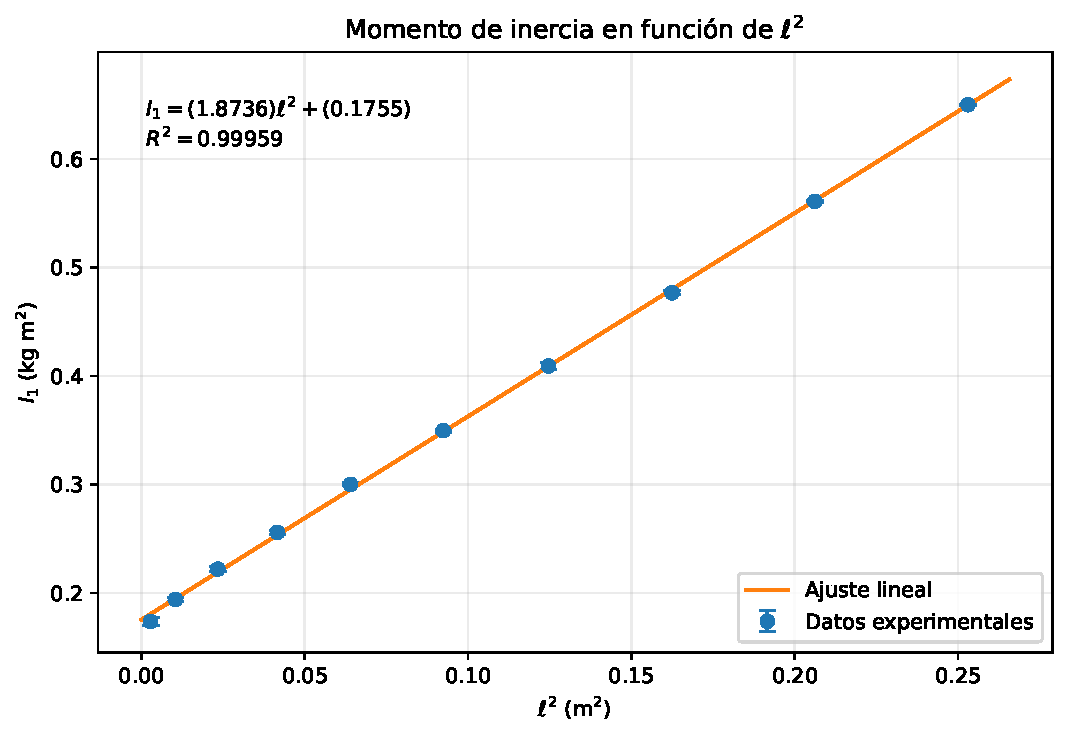
\includegraphics[width=0.72\textwidth]
    {../figuras/inercia_vs_distancia2_integrante1.pdf}
    \caption{Momento de inercia $I_1$ en función de $\ell^2$ para el primer conjunto de datos.}
    \label{fig:steiner_integrante1}
\end{figure}

El ajuste lineal realizado mediante Python fue

\[
\boxed{
I_1=1.873578\,\ell^2+0.175516
}
\]

con

\[
\boxed{
R^2=0.999588
}.
\]

Comparando esta expresión con

\[
I_1=M\ell^2+I_G,
\]

se obtuvo

\[
\boxed{
M_{\mathrm{exp}}
=
(1.87358\pm0.01344)\,\mathrm{kg}
}
\]

y

\[
\boxed{
I_{G,\mathrm{exp}}
=
(0.17552\pm0.00172)\,\mathrm{kg\,m^2}
}.
\]

\subsection{Resultados de los demás conjuntos de datos}

Los conjuntos de datos correspondientes a los integrantes 2 y 3 fueron
procesados mediante el mismo procedimiento desarrollado anteriormente.

Las gráficas correspondientes a estos dos conjuntos de datos se presentan en la sección de Anexos, donde se incluyen las representaciones de $T$ en función de $\ell$ y de $I_1$ en función de $\ell^2$.

Los resultados obtenidos se presentan a continuación.

\begin{table}[H]
    \centering
    \small
    \renewcommand{\arraystretch}{1.05}
    \setlength{\tabcolsep}{7pt}

    \begin{tabular}{ccccc}
        \toprule
        \textbf{Hueco} &
        $\boldsymbol{\ell}$ \textbf{(m)} &
        $\boldsymbol{T^2}$ \textbf{(s$^2$)} &
        $\boldsymbol{I_1}$ \textbf{(kg\,m$^2$)} &
        $\boldsymbol{\ell^2}$ \textbf{(m$^2$)} \\
        \midrule
        1  & 0.503 & 2.7883 & 0.6413 & 0.253009 \\
        2  & 0.454 & 2.6891 & 0.5583 & 0.206116 \\
        3  & 0.403 & 2.6417 & 0.4868 & 0.162409 \\
        4  & 0.353 & 2.5472 & 0.4112 & 0.124609 \\
        5  & 0.304 & 2.5728 & 0.3576 & 0.092416 \\
        6  & 0.253 & 2.6077 & 0.3017 & 0.064009 \\
        7  & 0.204 & 2.7689 & 0.2583 & 0.041616 \\
        8  & 0.153 & 3.0508 & 0.2134 & 0.023409 \\
        9  & 0.102 & 4.1875 & 0.1953 & 0.010404 \\
        10 & 0.053 & 7.2289 & 0.1752 & 0.002809 \\
        \bottomrule
    \end{tabular}

    \caption{Resultados calculados para el segundo conjunto de datos.}
    \label{tab:resultados_integrante2}
\end{table}

\begin{table}[H]
    \centering
    \small
    \renewcommand{\arraystretch}{1.05}
    \setlength{\tabcolsep}{7pt}

    \begin{tabular}{ccccc}
        \toprule
        \textbf{Hueco} &
        $\boldsymbol{\ell}$ \textbf{(m)} &
        $\boldsymbol{T^2}$ \textbf{(s$^2$)} &
        $\boldsymbol{I_1}$ \textbf{(kg\,m$^2$)} &
        $\boldsymbol{\ell^2}$ \textbf{(m$^2$)} \\
        \midrule
        1  & 0.503 & 2.6765 & 0.6156 & 0.253009 \\
        2  & 0.454 & 2.4118 & 0.5007 & 0.206116 \\
        3  & 0.403 & 2.6077 & 0.4805 & 0.162409 \\
        4  & 0.353 & 2.5403 & 0.4100 & 0.124609 \\
        5  & 0.304 & 2.5493 & 0.3544 & 0.092416 \\
        6  & 0.253 & 2.5520 & 0.2952 & 0.064009 \\
        7  & 0.204 & 2.7733 & 0.2587 & 0.041616 \\
        8  & 0.153 & 2.9435 & 0.2059 & 0.023409 \\
        9  & 0.102 & 4.1738 & 0.1947 & 0.010404 \\
        10 & 0.053 & 7.2990 & 0.1769 & 0.002809 \\
        \bottomrule
    \end{tabular}

    \caption{Resultados calculados para el tercer conjunto de datos.}
    \label{tab:resultados_integrante3}
\end{table}

Finalmente, los parámetros obtenidos mediante el ajuste lineal de
$I_1$ en función de $\ell^2$ para los tres conjuntos de datos fueron:

\begin{table}[H]
    \centering
    \small
    \renewcommand{\arraystretch}{1.15}

    \begin{tabular}{cccc}
        \toprule
        \textbf{Conjunto} &
        $\boldsymbol{M_{\mathrm{exp}}}$ \textbf{(kg)} &
        $\boldsymbol{I_{G,\mathrm{exp}}}$ \textbf{(kg\,m$^2$)} &
        $\boldsymbol{R^2}$ \\
        \midrule

        1 &
        $1.87358\pm0.01344$ &
        $0.17552\pm0.00172$ &
        0.999588 \\

        2 &
        $1.86286\pm0.02479$ &
        $0.17720\pm0.00317$ &
        0.998585 \\

        3 &
        $1.71462\pm0.06721$ &
        $0.18110\pm0.00859$ &
        0.987857 \\

        \bottomrule
    \end{tabular}

    \caption{Resultados de los ajustes lineales para los tres conjuntos de datos.}
    \label{tab:resultados_tres_integrantes}
\end{table}

\newpage
\section{Discusión}

Los resultados experimentales muestran que el período del péndulo físico depende de la distancia $\ell$ entre el eje de suspensión y el centro de masa. Para el primer conjunto de datos, el período disminuyó conforme el eje se aproximó al centro de masa hasta alcanzar un mínimo experimental de $1.5860\,\mathrm{s}$ para $\ell=0.304\,\mathrm{m}$, y posteriormente aumentó al continuar disminuyendo dicha distancia. Este comportamiento concuerda cualitativamente con la dependencia teórica del período de un péndulo físico.

A partir del modelo teórico se obtuvo una distancia correspondiente al período mínimo de
$\ell_{\min}=0.289161\,\mathrm{m}$ y un período mínimo de
$T_{\min}=1.525564\,\mathrm{s}$. La diferencia con el mínimo experimental puede atribuirse, entre otros factores, a que las posiciones del eje de suspensión están determinadas por los agujeros discretos de la barra; por tanto, no fue posible realizar una medición exactamente en la posición teórica del mínimo.

La representación de $I_1$ en función de $\ell^2$ presentó un comportamiento aproximadamente lineal, de acuerdo con la relación de Steiner
\[
I_1=I_G+M\ell^2.
\]
Para el primer conjunto se obtuvo $R^2=0.999588$, mientras que para el segundo y tercer conjunto se obtuvieron $R^2=0.998585$ y $R^2=0.987857$, respectivamente. Estos valores muestran una fuerte correspondencia entre los datos experimentales y la dependencia lineal predicha por el teorema de Steiner.

La masa determinada mediante la pendiente del ajuste fue
$M_{\mathrm{exp}}=(1.87358\pm0.01344)\,\mathrm{kg}$ para el primer conjunto y
$M_{\mathrm{exp}}=(1.86286\pm0.02479)\,\mathrm{kg}$ para el segundo, valores próximos a la masa medida directamente, $M=1.8402\,\mathrm{kg}$. En el tercer conjunto se obtuvo
$M_{\mathrm{exp}}=(1.71462\pm0.06721)\,\mathrm{kg}$, observándose una mayor desviación y dispersión respecto de los otros conjuntos.

Para el momento de inercia respecto del centro de masa se obtuvieron
$0.17552\,\mathrm{kg\,m^2}$,
$0.17720\,\mathrm{kg\,m^2}$ y
$0.18110\,\mathrm{kg\,m^2}$ para los tres conjuntos, respectivamente. Estos valores son superiores al valor teórico
$I_{G,\mathrm{teo}}=0.153867\,\mathrm{kg\,m^2}$. Esta diferencia puede estar asociada a las aproximaciones del modelo empleado, ya que la expresión teórica considera una barra rectangular homogénea, mientras que la barra experimental posee múltiples perforaciones que modifican su distribución de masa. Asimismo, pueden contribuir efectos como la fricción en el punto de suspensión, la determinación de $\ell$ y la incertidumbre asociada al cronometraje manual.

En conjunto, la elevada linealidad obtenida en las gráficas de $I_1$ frente a $\ell^2$ respalda experimentalmente la relación establecida por el teorema de Steiner, aunque las diferencias encontradas en $I_G$ evidencian las limitaciones del modelo ideal y de las condiciones experimentales.

\newpage
\section{Conclusiones}

\begin{enumerate}

    \item Se determinó experimentalmente la dependencia del período de oscilación del péndulo físico con la distancia entre el eje de suspensión y el centro de masa. Para el primer conjunto de datos se obtuvo un período mínimo medido de
    $T_{\min}=1.5860\,\mathrm{s}$ en $\ell=0.304\,\mathrm{m}$, próximo a la posición teórica del mínimo,
    $\ell_{\min}=0.289161\,\mathrm{m}$.

    \item La representación de $I_1$ en función de $\ell^2$ presentó un comportamiento lineal para los tres conjuntos experimentales, obteniéndose coeficientes de determinación de
    $R^2=0.999588$, $0.998585$ y $0.987857$. Este comportamiento es consistente con la relación
    $I_1=I_G+M\ell^2$ establecida por el teorema de Steiner.

    \item A partir de las pendientes de los ajustes lineales se obtuvieron masas experimentales de
    $1.87358\,\mathrm{kg}$,
    $1.86286\,\mathrm{kg}$ y
    $1.71462\,\mathrm{kg}$ para los tres conjuntos de datos, respectivamente. Los dos primeros resultados presentan mayor proximidad a la masa medida directamente de la barra,
    $M=1.8402\,\mathrm{kg}$.

    \item Los momentos de inercia respecto del centro de masa determinados experimentalmente fueron
    $0.17552\,\mathrm{kg\,m^2}$,
    $0.17720\,\mathrm{kg\,m^2}$ y
    $0.18110\,\mathrm{kg\,m^2}$, mientras que el modelo de barra rectangular homogénea proporciona
    $I_{G,\mathrm{teo}}=0.153867\,\mathrm{kg\,m^2}$. La diferencia observada evidencia las limitaciones del modelo ideal para representar una barra real perforada, además de las incertidumbres asociadas al procedimiento experimental.

    \item En conjunto, los resultados permitieron determinar experimentalmente los momentos de inercia asociados a diferentes ejes de suspensión y comprobar la dependencia lineal entre $I_1$ y $\ell^2$ predicha por el teorema de Steiner.

\end{enumerate}

\newpage
\section{Bibliografía}
\begin{thebibliography}{99}

\bibitem{alonso_finn}
Alonso, M. y Finn, E. J. (1995).
\textit{Física}.
Addison-Wesley Iberoamericana.

\bibitem{sears}
Young, H. D. y Freedman, R. A.
\textit{Física universitaria con física moderna}.
Pearson Educación.

\bibitem{serway}
Serway, R. A. y Jewett, J. W.
\textit{Física para ciencias e ingeniería}.
Cengage Learning.

\bibitem{giancoli}
Giancoli, D. C.
\textit{Física: principios con aplicaciones}.
Pearson Educación.

\bibitem{tipler}
Tipler, P. A. y Mosca, G.
\textit{Física para la ciencia y la tecnología}.
Editorial Reverté.

\bibitem{guia_lab}
Universidad Nacional de Ingeniería, Facultad de Ciencias.
\textit{Laboratorio 9: Péndulo físico y teorema de Steiner}.
Guía de Laboratorio de Física II, 2026.

\end{thebibliography}

\newpage
\section{Anexos}

\subsection{Repositorio del laboratorio}

Los archivos utilizados para el procesamiento de los datos experimentales,
la elaboración de las gráficas y el desarrollo del informe se encuentran
disponibles en el repositorio de GitHub del laboratorio:

\begin{center}
    \url{https://github.com/alexandradeOz-wq/FISICA-2-LABORATORY}
\end{center}

El repositorio contiene los datos experimentales, los códigos desarrollados
en Python para el procesamiento y análisis de las mediciones, las gráficas
obtenidas y el código fuente en \LaTeX{} empleado para la elaboración del
presente informe.

\subsection{Participación de los integrantes}

El desarrollo de la experiencia fue realizado de manera conjunta por los
tres integrantes. Las principales actividades desarrolladas por cada uno
se resumen en el siguiente cuadro.

\begin{table}[H]
    \centering
    \small
    \renewcommand{\arraystretch}{1.25}
    \setlength{\tabcolsep}{8pt}

    \begin{tabular}{
        >{\raggedright\arraybackslash}p{0.30\textwidth}
        >{\raggedright\arraybackslash}p{0.62\textwidth}
    }
        \toprule

        \textbf{Integrante} &
        \textbf{Participación} \\

        \midrule

        Moreno Cabanillas, Alexandra Romina &
        Participación en el montaje y ejecución de la experiencia,
        registro de los tiempos de oscilación y distancias experimentales,
        procesamiento computacional de los datos mediante Python,
        elaboración de gráficas y participación en la redacción y revisión
        del informe. \\

        \addlinespace

        Polak Mory, Mauricio Andre &
        Participación en el montaje y ejecución de la experiencia,
        medición de los tiempos de oscilación y dimensiones de la barra,
        organización y verificación de los datos experimentales,
        análisis de los resultados y participación en la redacción y
        revisión del informe. \\

        \addlinespace

        Cárdenas Loyola, Pablo Mauro &
        Participación en el montaje y ejecución de la experiencia,
        medición de los tiempos de oscilación y posición de los ejes de
        suspensión, verificación de los cálculos experimentales,
        interpretación de los resultados y participación en la redacción
        y revisión del informe. \\

        \bottomrule
    \end{tabular}

    \caption{Participación de los integrantes en el desarrollo del laboratorio.}
    \label{tab:participacion_integrantes}
\end{table}

\subsection{Gráficas complementarias}

Las siguientes gráficas corresponden a los conjuntos de datos de los
integrantes 2 y 3, procesados mediante el mismo procedimiento empleado
para el primer conjunto.

\subsubsection*{Integrante 2}

\begin{figure}[H]
    \centering
    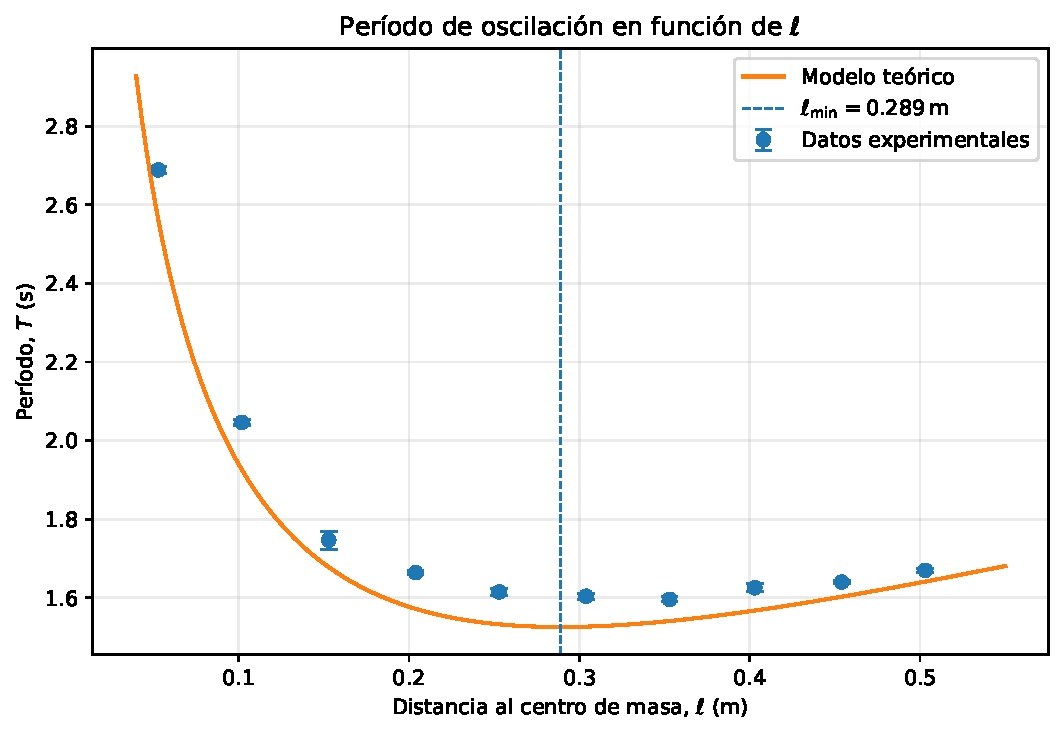
\includegraphics[width=0.62\textwidth]
    {../figuras/periodo_vs_distancia_integrante2.pdf}
    \caption{Período de oscilación en función de $\ell$ para el segundo conjunto de datos.}
    \label{fig:periodo_integrante2}
\end{figure}

\begin{figure}[H]
    \centering
    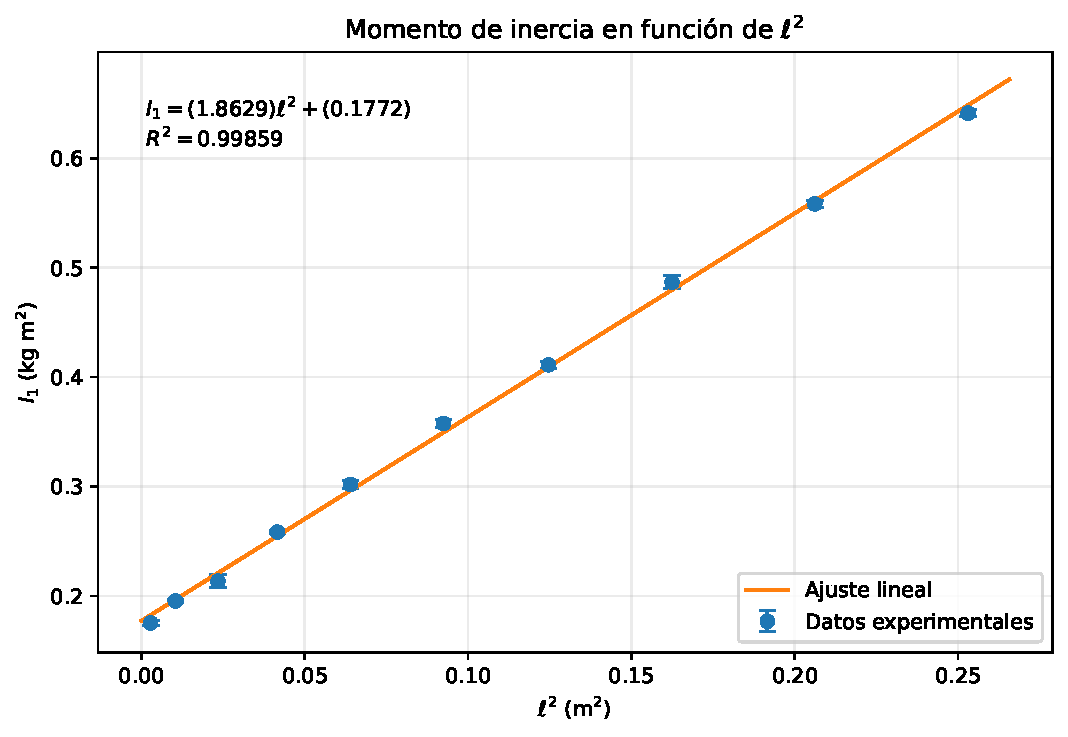
\includegraphics[width=0.62\textwidth]
    {../figuras/inercia_vs_distancia2_integrante2.pdf}
    \caption{Momento de inercia $I_1$ en función de $\ell^2$ para el segundo conjunto de datos.}
    \label{fig:inercia_integrante2}
\end{figure}

\subsubsection*{Integrante 3}

\begin{figure}[H]
    \centering
    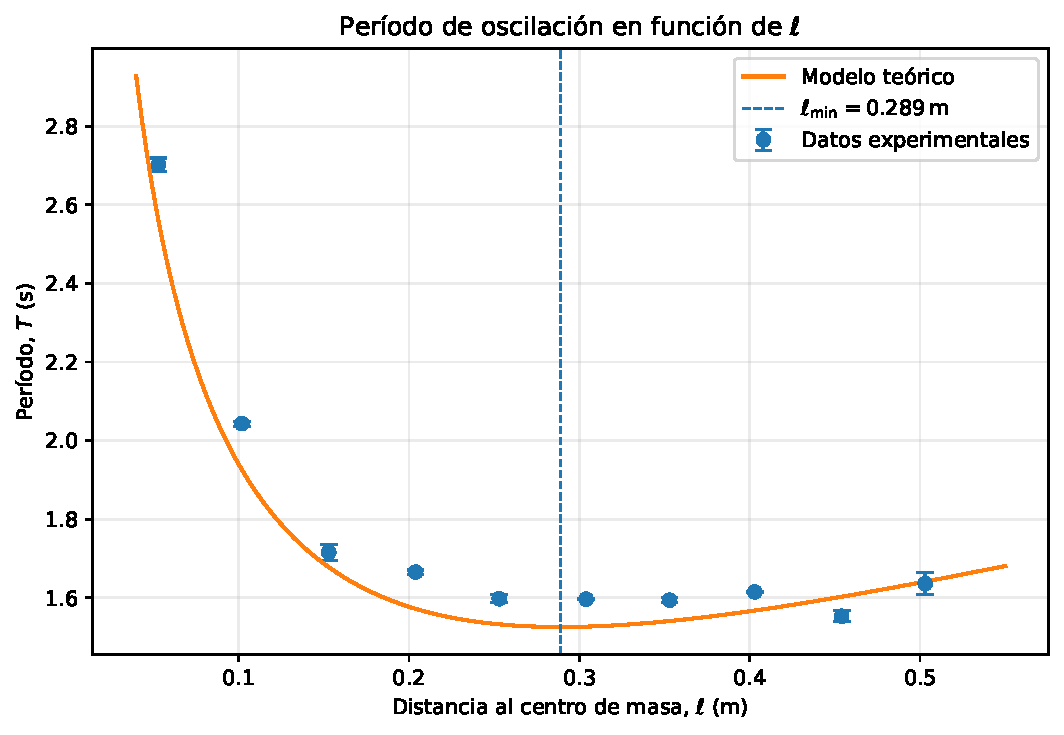
\includegraphics[width=0.62\textwidth]
    {../figuras/periodo_vs_distancia_integrante3.pdf}
    \caption{Período de oscilación en función de $\ell$ para el tercer conjunto de datos.}
    \label{fig:periodo_integrante3}
\end{figure}

\begin{figure}[H]
    \centering
    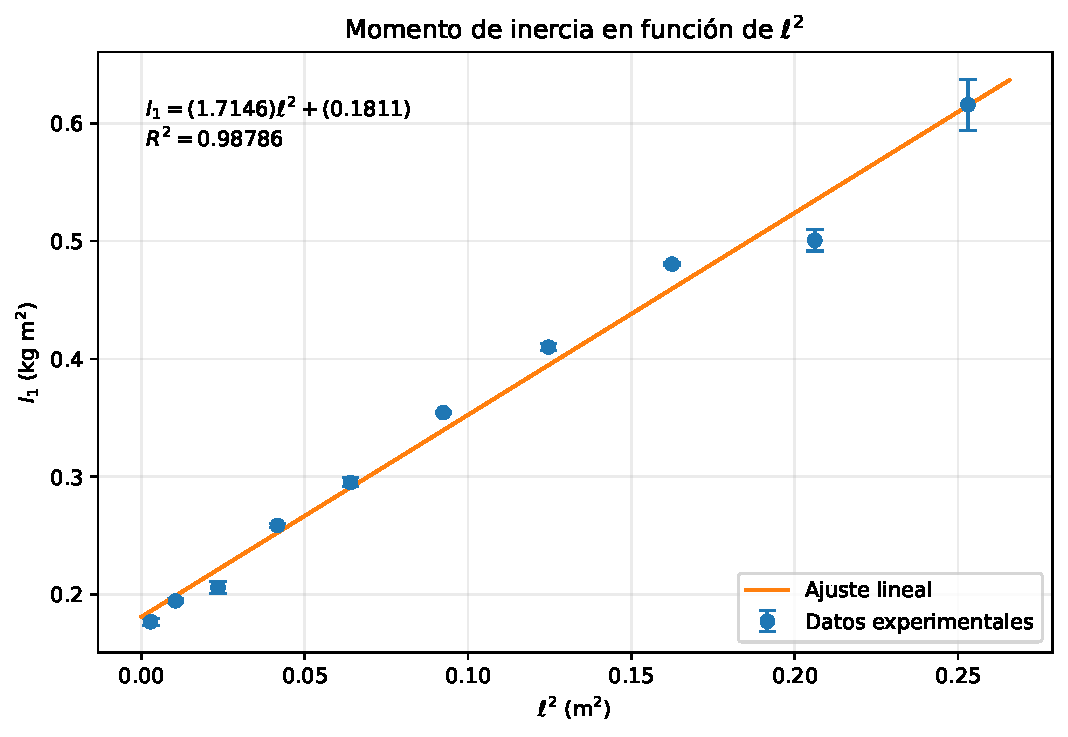
\includegraphics[width=0.62\textwidth]
    {../figuras/inercia_vs_distancia2_integrante3.pdf}
    \caption{Momento de inercia $I_1$ en función de $\ell^2$ para el tercer conjunto de datos.}
    \label{fig:inercia_integrante3}
\end{figure}

\end{document}